%!TEX ROOT = sample-thesis.tex
\chapter{Introduction}

So this is the preamble at the beginning of the chapter. The purpose may be to introduce the themes of the chapter and main headings.

So this is a second paragraph.

\section{First Test and I need a really long title, please do oblige me won't you? Just a few more words and yes we're there}
\lipsum[1-2]

\begin{figure}[hbt!]\centering

\includegraphics[width=.3\textwidth]{green}
\caption[First figure]{First figure\\\source{Somewhere from the Web.}}

\bigskip


\includegraphics[width=.3\textwidth]{school}
\caption{Second figure. Now I need a long caption to test out how things look in the List of Figures. Is this long enough yet? Is it? Is it?}
\end{figure}

\lipsum[4-5]

\begin{figure}[hbt!]
\centering
%
\begin{minipage}{0.3\textwidth}
\centering

\includegraphics[width=\linewidth]{green}
\subcaption{The first subfigure}
\end{minipage}
%
\hspace{1cm}
%
\begin{minipage}{0.3\textwidth}
\centering

\includegraphics[width=\linewidth]{school}
\subcaption{The second subfigure}
\end{minipage}

\caption{An example with subfigures}
\end{figure}

\subsection{Second Test}
Their \cite{audibert:2004} requirements\footnote{See here, how weird, how to fill out an entire line. See here, how weird, how to fill out an entire line. See here, how weird, how to fill out an entire line. See here, how weird, how to fill out an entire line. See here, how weird, how to fill out an entire line. } are really amazing\footnote{don't you agree?} \cite[34]{budanitsky:hirst:2006}.

Looks like everyting's working. 

\subsubsection{A Subsubsection}

Not a good idea. Really.

\subsubsection{Another Subsubsection}

Not a good idea. Really.

\begin{photo}[hbt!]
\centering
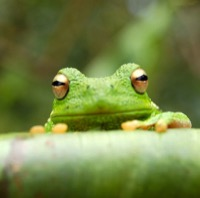
\includegraphics[width=.5\linewidth]{frog}
\caption{This is a photograph}
\end{photo}

\subsection{This is another Subsection}

Dummy text! \lipsum[1]

\section{Yeah}

And here's a long quotation, it should be an indented block and single-spaced:

\begin{quote}
\lipsum[5-6]
\end{quote}

Time for some maths, and later there's a table.

\begin{equation}
\left[M\frac{\partial }{\partial M}+\beta(g)\frac{\partial }{\partial g}+n\gamma\right] G^{(n)}(x_1,x_2,\ldots,x_n;M,g)=0
\end{equation}

\begin{table}[hbt!]
\caption{This is a table}
\centering
\begin{tabular}{ l c r }
\hline
Hey & How's it & Going?\\ \hline
Fine! & Just great. & See ya!\\
Fine! & Just great. & See ya!\\
\hline
\end{tabular}

\source{The Source.}
\end{table}

\lipsum[7]